\setstretch{2} % double spacing for proofs

% Legacy equation-by-equation proof blocks were removed so that the appendix
% now tracks the current main-text results one-for-one.

\subsubsection{One-Sample Mean Results}
\label{sec:proofs-one-sample}

\paragraph{Proof of Proposition~\ref{prop:ppi-var} (Mean PPI/PPI++ Variance)}
\label{sec:proof-vanilla-var}
This proof covers both the PPI and \texttt{PPI++} variance results stated in Proposition~\ref{prop:ppi-var}.

Write
\[
\wh{\theta}_{\mathrm{PPI}}
= \bar f_U + (\bar Y_L-\bar f_L),
\qquad
\wh{\theta}_\lambda
= \bar Y_L + \lambda(\bar f_U-\bar f_L),
\]
where $\bar f_U = N^{-1}\sum_{j=1}^N \wt f_j$,
$\bar f_L = n^{-1}\sum_{i=1}^n f_i$, and
$\bar Y_L = n^{-1}\sum_{i=1}^n Y_i$.
Because the labeled and unlabeled splits are independent and drawn from the
same covariate distribution,
\[
\E[\bar f_U]=\E[\bar f_L]=\E[f(X)],
\]
so
\[
\E[\wh{\theta}_{\mathrm{PPI}}]
= \E[f(X)] + \E[Y-f(X)]
= \theta^\star,
\qquad
\E[\wh{\theta}_\lambda]=\theta^\star
\]
for every fixed $\lambda$.

For vanilla PPI, independence of the labeled and unlabeled terms gives
\[
\Var(\wh{\theta}_{\mathrm{PPI}})
= \Var(\bar f_U) + \Var(\bar Y_L-\bar f_L)
= \frac{\sigma_f^2}{N} + \frac{\sigma_\varepsilon^2}{n},
\]
which is~\eqref{eq:ppi-var}.

For \texttt{PPI++},
\[
\Var(\wh{\theta}_\lambda)
= \Var(\bar Y_L) + \lambda^2\Var(\bar f_U-\bar f_L)
+ 2\lambda\,\Cov(\bar Y_L,\bar f_U-\bar f_L).
\]
Now $\Var(\bar Y_L)=\sigma_Y^2/n$,
$\Var(\bar f_U-\bar f_L)=\sigma_f^2/N+\sigma_f^2/n$, and
$\Cov(\bar Y_L,\bar f_U)=0$ by split independence, while
$\Cov(\bar Y_L,\bar f_L)=\Cov(Y,f)/n$.
Substituting these identities yields
\[
\Var(\wh{\theta}_\lambda)
=
\frac{\sigma_Y^2}{n}
+ \lambda^2\!\left(\frac{\sigma_f^2}{N}+\frac{\sigma_f^2}{n}\right)
- \frac{2\lambda\,\Cov(Y,f)}{n},
\]
which is~\eqref{eq:ppi++-variance}. Joint asymptotic normality follows from the
multivariate central limit theorem applied to the labeled and unlabeled sample
means.

\paragraph{Justification of the Classical Power Approximation}
\label{sec:proof-vanilla-power}
Under the alternative $\theta^\star=\theta_0+\Delta$, the classical Wald
statistic is asymptotically normal with mean
$\Delta/(\sigma_Y/\sqrt{n})$ and variance $1$, so the exact two-sided normal
approximation is~\eqref{eq:classical-power}. The second term in that display,
\[
\Phi\!\left(-z_{1-\alpha/2}-\frac{|\Delta|}{\sigma_Y/\sqrt{n}}\right),
\]
is always no larger than the first and becomes negligible once the noncentrality
$|\Delta|/(\sigma_Y/\sqrt{n})$ is moderate. Dropping it yields the usual
planning approximation
$|\Delta|/(\sigma_Y/\sqrt{n}) \ge z_{1-\alpha/2}+z_{1-\beta}$, or equivalently
$\sigma_Y^2/n \le S^2$, which is the inversion used in the main text.

\paragraph{Proof of Equations~\eqref{eq:lambda-star} and~\eqref{eq:ppi++-var-opt}}
Given~\eqref{eq:ppi++-variance},
\[
g(\lambda)
= \Var(\wh{\theta}_\lambda)
= \frac{\sigma_Y^2}{n}
+ \lambda^2\!\left(\frac{\sigma_f^2}{N}+\frac{\sigma_f^2}{n}\right)
- \frac{2\lambda\,\Cov(Y,f)}{n}.
\]
This is a convex quadratic in $\lambda$, so its minimizer satisfies
\[
g'(\lambda)
= 2\lambda\!\left(\frac{\sigma_f^2}{N}+\frac{\sigma_f^2}{n}\right)
- \frac{2\Cov(Y,f)}{n}
= 0.
\]
Solving gives
\[
\lambda^\star
= \frac{\Cov(Y,f)}{\sigma_f^2(1+n/N)}
= \frac{\Cov(Y,f)}{(1+r)\sigma_f^2},
\]
which is~\eqref{eq:lambda-star}. Substituting this value back into
\eqref{eq:ppi++-variance} yields
\[
\Var(\wh{\theta}_{\lambda^\star})
= \frac{\sigma_Y^2}{n}
- \frac{\Cov(Y,f)^2}{\sigma_f^2}\cdot \frac{N}{n(n+N)},
\]
which is~\eqref{eq:ppi++-var-opt}.

\paragraph{Proof of Proposition~\ref{prop:ppi++-power} (\texttt{PPI++} Power)}
Under $\theta^\star=\theta_0+\Delta$,
\[
Z
= \frac{\wh{\theta}_{\lambda^\star}-\theta_0}
{\sqrt{\Var(\wh{\theta}_{\lambda^\star})}}
\;\dot{\sim}\;
\mathcal N\!\left(
\frac{\Delta}{\sqrt{\Var(\wh{\theta}_{\lambda^\star})}},\,1
\right),
\]
so the two-sided rejection probability is
\[
P(|Z|\ge z_{1-\alpha/2})
=
\Phi\!\left(-z_{1-\alpha/2}
+ \frac{|\Delta|}{\sqrt{\Var(\wh{\theta}_{\lambda^\star})}}\right)
+ \Phi\!\left(-z_{1-\alpha/2}
- \frac{|\Delta|}{\sqrt{\Var(\wh{\theta}_{\lambda^\star})}}\right),
\]
which is exactly~\eqref{eq:ppi++-power}.

\paragraph{Proof of Proposition~\ref{prop:ppi++-n} (Sample Size Inversion)}
\label{sec:proof-ppi++-n}
From Proposition~\ref{prop:ppi++-power}, achieving target power is ensured by
\[
\Var(\wh{\theta}_{\lambda^\star}) \le S^2,
\qquad
S^2 = \frac{\Delta^2}{(z_{1-\alpha/2}+z_{1-\beta})^2}.
\]
Substituting~\eqref{eq:ppi++-var-opt} gives
\[
\frac{\sigma_Y^2}{n}
- \frac{\Cov(Y,f)^2}{\sigma_f^2}\cdot\frac{N}{n(n+N)}
\le S^2.
\]
Multiplying by $n(n+N)>0$ and using
$\rho_{Yf}^2=\Cov(Y,f)^2/(\sigma_Y^2\sigma_f^2)$ yields
\[
S^2 n^2 + (S^2N-\sigma_Y^2)n - N\sigma_Y^2(1-\rho_{Yf}^2)\ge 0.
\]
Since this quadratic opens upward, the feasible region is $n$ greater than or
equal to its positive root:
\[
n \ge
\frac{\sigma_Y^2 - S^2 N
+ \sqrt{(\sigma_Y^2 - S^2 N)^2
+ 4 S^2 N \sigma_Y^2 (1-\rho_{Yf}^2)}}{2S^2},
\]
which is~\eqref{eq:ppi++-n-formula}.

\paragraph{Proof of Corollary~\ref{cor:rule-of-thumb} (Rule of Thumb)}
When $N \gg n$, we have $N/(n+N)=1+o(1)$ and therefore
\[
\Var(\wh{\theta}_{\lambda^\star})
= \frac{\sigma_Y^2}{n}
- \frac{\Cov(Y,f)^2}{\sigma_f^2}\cdot\frac{1+o(1)}{n}
= \frac{\sigma_Y^2(1-\rho_{Yf}^2)}{n} + o(n^{-1}).
\]
The classical variance is $\sigma_Y^2/n$, so to first order the required
labeled sample size scales by the same factor, giving
$n_{\mathrm{PPI}}/n_{\mathrm{cl}} \approx 1-\rho_{Yf}^2$.

\subsubsection{Two-Sample, Paired, and Contingency-Table Extensions}
\label{sec:proofs-extensions}

\paragraph{Proof of Proposition~\ref{prop:ttest-var} (Two-Sample Variance)}
\label{sec:proof-ttest}
From the definition~\eqref{eq:ppi++-ttest-est},
\[
\wh{\Delta}_{\mathrm{PPI}}
= \wh{\theta}_{A,\mathrm{PPI}}-\wh{\theta}_{B,\mathrm{PPI}}.
\]
Applying the one-sample oracle-variance formula~\eqref{eq:ppi++-var-opt}
within each group gives
\[
\Var(\wh{\theta}_{g,\lambda_g^\star})
=
\frac{\sigma_{Y,g}^2}{n_g}
- \frac{\Cov(Y_g,f_g)^2}{\sigma_{f,g}^2}
\cdot \frac{N_g}{n_g(n_g+N_g)},
\qquad g\in\{A,B\}.
\]
Because the two groups are independent, the cross-covariance vanishes, so
\[
\Var(\wh{\Delta}_{\mathrm{PPI}})
= \Var(\wh{\theta}_{A,\lambda_A^\star})
+ \Var(\wh{\theta}_{B,\lambda_B^\star}),
\]
which is exactly~\eqref{eq:ppi++-ttest-var}. The approximation
\eqref{eq:ppi++-ttest-var-approx} follows from
$\Cov(Y_g,f_g)^2/\sigma_{f,g}^2 = \sigma_{Y,g}^2\Corr(Y_g,f_g)^2$ and
$N_g/(n_g+N_g)=1+O(n_g/N_g)$.

\paragraph{Proof of Proposition~\ref{prop:paired-var} (Paired Variance)}
Let $D=Y^A-Y^B$ and $G=f^A-f^B$. The paired \texttt{PPI++} estimator is exactly
the one-sample \texttt{PPI++} estimator applied to the paired differences, with
target parameter $\E[D]$ and surrogate $G$. Proposition~\ref{prop:ppi-var}
therefore gives
\[
\Var(\wh{\Delta}_{\mathrm{PPI++}})
= \frac{\Var(D)}{n}
- \frac{\Cov(D,G)^2}{\Var(G)}\cdot \frac{N}{n(n+N)}.
\]
Rewriting $\Cov(D,G)^2/\Var(G)=\Var(D)\Corr(D,G)^2$ gives the equivalent form in
the proposition, and letting $N\gg n$ yields the displayed approximation.

\paragraph{Proof of Proposition~\ref{prop:2x2-n} ($2\times2$ Sample Size)}
For each group $g\in\{0,1\}$, the event-rate estimator
\[
\wh p_{g,\lambda_g}
= \bar Y_{L,g} + \lambda_g(\bar f_{U,g}-\bar f_{L,g})
\]
is a one-sample \texttt{PPI++} estimator for the binary mean $p_g$. Since
$Y_g\in\{0,1\}$, $\Var(Y_g)=p_g(1-p_g)$, and in the regime $N_g\gg n_g$,
Corollary~\ref{cor:rule-of-thumb} gives
\[
\Var(\wh p_{g,\lambda_g^\star})
\approx \frac{p_g(1-p_g)(1-\rho_g^2)}{n_g}.
\]

For $\log(\mathrm{RR})=\log p_1-\log p_0$, the gradient with respect to
$(p_0,p_1)$ is $(-1/p_0,\;1/p_1)^\top$. Since the two groups are independent,
the delta method yields
\[
\Var(\log \widehat{\mathrm{RR}})
\approx
\frac{\Var(\wh p_{0,\lambda_0^\star})}{p_0^2}
+ \frac{\Var(\wh p_{1,\lambda_1^\star})}{p_1^2}
=
\frac{1}{n_0}\frac{(1-p_0)(1-\rho_0^2)}{p_0}
+ \frac{1}{n_1}\frac{(1-p_1)(1-\rho_1^2)}{p_1}.
\]
Substituting $n_1=\kappa n_0$ gives the first displayed variance formula in the
proposition.

For $\log(\mathrm{OR})=\operatorname{logit}(p_1)-\operatorname{logit}(p_0)$, the
gradient is
$(-[p_0(1-p_0)]^{-1},\; [p_1(1-p_1)]^{-1})^\top$, so the same argument gives
\[
\Var(\log \widehat{\mathrm{OR}})
\approx
\frac{1}{n_0}\frac{1-\rho_0^2}{p_0(1-p_0)}
+ \frac{1}{n_1}\frac{1-\rho_1^2}{p_1(1-p_1)}.
\]
The sample-size expressions follow by imposing
$\Var(\log \widehat{\mathrm{RR}})\le S_{\mathrm{RR}}^2$ and
$\Var(\log \widehat{\mathrm{OR}})\le S_{\mathrm{OR}}^2$ and then solving for
$n_0$; the balanced-design formulas set $\kappa=1$. Setting
$\rho_0=\rho_1=0$ recovers the usual classical formulas.

% --------------------------------------------------------------------------
% NOTE: The cross-fitting proof below is stated directly in the one-sample
% mean notation of the main text so that the appendix is self-contained.
% --------------------------------------------------------------------------
\subsubsection{Cross-Fitted PPI++ Distribution}
\label{sec:proof-cross-fitting}

We state the cross-fitting result directly for the one-sample mean problem of
Sections~\ref{sec:ppi-vanilla}--\ref{sec:ppi++}. Partition the labeled sample
into folds $I_1,\ldots,I_K$, let $f^{(j)}$ denote the predictor trained
without fold $I_j$, and define the cross-fitted \texttt{PPI++} estimator
\[
\wh{\theta}_{\lambda,\mathrm{cf}}
=
\bar Y_L
+
\lambda\left(
\frac{1}{K}\sum_{j=1}^K \bar f_{U}^{(j)}
-
\frac{1}{n}\sum_{j=1}^K\sum_{i\in I_j} f^{(j)}(X_i)
\right),
\qquad
\bar f_U^{(j)} = \frac{1}{N}\sum_{m=1}^N f^{(j)}(\wt X_m).
\]
This is the same rectified mean estimator as in~\eqref{eq:ppi++-estimator},
except that each labeled observation is evaluated by a predictor that was not
trained on its own fold.

\begin{assumption}[Prediction stability]\label{ass:M-stable-f}
The predictors $f^{(1)},\ldots,f^{(K)}$ trained on the $K$ folds satisfy
$\|f^{(j)} - \bar f\|_2 = o_P(1)$ as $n \to \infty$,
where $\bar f = K^{-1}\sum_{j=1}^K f^{(j)}$ is the average predictor.
\end{assumption}

Lemmas~3--4 in the proof of Theorem~2 of~\citet{zrnic2024cross}, specialized
to the scalar mean estimating function $\ell_\theta(Y,X)=Y-\theta$, imply
that the fold-specific prediction averages can be replaced by the average
predictor $\bar f$ without affecting the estimator at the $n^{-1/2}$ scale:
\begin{align*}
\frac{1}{K}\sum_{j=1}^K \bar f_U^{(j)}
&=
\frac{1}{N}\sum_{m=1}^N \bar f(\wt X_m) + o_P(n^{-1/2}), \\
\frac{1}{n}\sum_{j=1}^K\sum_{i\in I_j} f^{(j)}(X_i)
&=
\frac{1}{n}\sum_{i=1}^n \bar f(X_i) + o_P(n^{-1/2}).
\end{align*}
Therefore
\[
\wh{\theta}_{\lambda,\mathrm{cf}}
=
\bar Y_L + \lambda(\bar f_{U,\bar f} - \bar f_{L,\bar f}) + o_P(n^{-1/2}),
\]
where
\[
\bar f_{U,\bar f} = \frac{1}{N}\sum_{m=1}^N \bar f(\wt X_m),
\qquad
\bar f_{L,\bar f} = \frac{1}{n}\sum_{i=1}^n \bar f(X_i).
\]

Conditional on the limiting predictor $\bar f$, this is exactly the same
algebraic form as the fixed-predictor estimator in
\eqref{eq:ppi++-estimator}, with $f$ replaced by $\bar f$. Since the labeled
and unlabeled samples are independent, the multivariate central limit theorem
gives
\[
\sqrt{n}\bigl(\wh{\theta}_{\lambda,\mathrm{cf}} - \theta^\star\bigr)
\overset{d}{\longrightarrow}
\mathcal N\!\left(
0,\;
\sigma_Y^2 + \lambda^2(1+r)\sigma_{\bar f}^2 - 2\lambda\,\Cov(Y,\bar f)
\right),
\]
where $r = \lim n/N$ and $\sigma_{\bar f}^2 = \Var(\bar f(X))$. Equivalently,
\[
\Var(\wh{\theta}_{\lambda,\mathrm{cf}})
=
\frac{\sigma_Y^2}{n}
+
\lambda^2\sigma_{\bar f}^2\!\left(\frac{1}{n}+\frac{1}{N}\right)
-
\frac{2\lambda\,\Cov(Y,\bar f)}{n}
+
o(n^{-1}).
\]
The oracle choice in this cross-fitted setting is therefore
\[
\lambda_{\mathrm{cf}}^\star
=
\frac{\Cov(Y,\bar f)}{(1+r)\sigma_{\bar f}^2},
\]
and substituting it into the variance expression yields the same first-order
formula as \eqref{eq:ppi++-var-opt}, again with $f$ replaced by the limiting
predictor $\bar f$.

\subsection{Supplementary Simulation Results}
\label{sec:appendix-sim-summary}

\iffalse
\begin{table}[!ht]
\centering\footnotesize
\begin{tabular}{@{}cclllp{4.0cm}@{}}
\toprule
\textbf{\#} & \textbf{\S} & \textbf{Experiment} & \textbf{Outcome} &
  \textbf{Test} & \textbf{Key parameters} \\
\midrule
1 & 5.1 & Mean (continuous) & Gaussian & One-sample &
  $n{\in}\{20{-}100\}$, $N{\in}\{200,500\}$,
  $\rho{\in}\{.5,.7,.9\}$ \\
2 & 5.1 & Mean (binary) & Bernoulli & One-sample &
  sens/spec ${\in}\{.70,.85,.95\}$ \\
3 & 5.1 & Two-sample (cont.) & Gaussian & Two-sample &
  $\Delta{=}0.3$ \\
4 & 5.1 & Two-sample (binary) & Bernoulli & Two-sample &
  $\Delta{=}0.08$ \\
5 & 5.1 & Paired (continuous) & Gaussian & Paired &
  $n{\in}\{20{-}100\}$ \\
6 & 5.1 & Paired (binary) & Bernoulli & Paired &
  $\rho_{\text{within}}{=}0.3$ \\
\midrule
7 & 5.2 & 2$\times$2 Table (OR \& RR) & Bernoulli & Contrast &
  $p_{\text{ctrl}}{=}0.20$, $p_{\text{exp}}{\in}\{.30,.35,.40\}$,
  acc${\in}\{70,80,90\}\%$, $N{\in}\{200,500\}$, $n{\in}\{20{-}100\}$ \\
8 & 5.2 & OLS regression & Gaussian & Contrast &
  $N{\in}\{200,500\}$, $n{\in}\{20{-}100\}$, $\rho{\in}\{.5,.7,.9\}$ \\
9 & 5.2 & GLM logistic & Bernoulli & Contrast &
  $N{\in}\{200,500\}$, accuracy${\in}\{70,80,90\}\%$, $n{\in}\{20{-}100\}$ \\
\midrule
10 & 5.3 & $n$-inversion & Mixed & --- &
  $N{=}500$, target power ${\in}\{.6,.7,.8,.9\}$ \\
11 & 5.3 & Rule of thumb & Gaussian & --- &
  $\rho{\in}[0.1,0.99]$, $N{\in}\{200,500,1{,}000,5{,}000\}$ \\
12 & 5.3 & Type~I error & Mixed & All &
  $\Delta{=}0$, $R{=}2{,}000$ \\
13 & 5.3 & $\lambda$ convergence & Gaussian & --- &
  $N{=}1{,}000$, $n{\in}\{20,50,100,200,500\}$ \\
\midrule
14 & 5.3 & Plugin $\lambda$ power & Gaussian & One-sample &
  $N{\in}\{200,500\}$, oracle vs.\ plugin $\hat\lambda$ \\
15 & 5.3 & Power vs.\ $\Delta$ & Gaussian & One-sample &
  $N{=}500$, $\Delta{\in}[0,0.5]$, $n{\in}\{20{-}100\}$ \\
16 & 5.3 & Small $n$ & Gaussian & One-sample &
  $N{\in}\{200,500\}$, $n{\in}\{15,20,25,30,50,100\}$, $R{=}2{,}000$ \\
17 & 5.3 & $N/n$ ratio & Gaussian & One-sample &
  $n{=}50$, $N/n{\in}\{1{-}100\}$ \\
18 & 5.3 & Unequal groups & Gaussian & Two-sample &
  $n_{\text{total}}{=}100$, $N_{\text{total}}{=}600$, same $A{:}B$ split for $n$ and $N$ \\
19 & 5.3 & Misspecified $\rho$ & Gaussian & One-sample &
  $N{=}500$, $\rho_{\text{plan}}{\neq}\rho_{\text{true}}$, $\rho_{\text{true}}$ truncated to $(0.01,0.99)$, $R{=}2{,}000$ \\
\midrule
20 & 5.3 & Log-normal (distributional robustness) & Log-normal & One-sample &
  Skewed; same grid as 1 \\
21 & 5.3 & $t$-distributed (distributional robustness) & $t_5$ & One-sample &
  Heavy-tailed; same grid as 1 \\
\bottomrule
\end{tabular}
\caption{Summary of all 21 simulation experiments, grouped by the
  main-text simulation subsections.}
\label{tab:simulation-settings}
\end{table}
\fi

\paragraph{Head-to-head planning comparison.}
Table~\ref{tab:head-to-head-multidesign} reorganizes representative
results from the main simulation settings into a single comparison
across one-sample, two-sample, and paired continuous designs.  It does
not introduce a new setting; rather, it summarizes the practical
tradeoffs between classical inference, vanilla PPI, and
\texttt{PPI++} (oracle and plugin) using common planning targets.

\begin{table}[!ht]
\centering
\caption{Head-to-head comparison across representative continuous
  planning scenarios (one-sample: $\Delta = 0.2$; two-sample:
  $\Delta = 0.3$; paired: $\Delta = 0.3$; all with $N = 5000$,
  $\rho = 0.7$, target power~$0.80$, $\alpha = 0.05$;
  MC $R = 5000$).  For plugin \texttt{PPI++}, planning uses the oracle
  closed-form $n$ and evaluates performance with
  plugin~$\hat\lambda$.}
\label{tab:head-to-head-multidesign}
\small
\begin{tabular}{llrrrr}
\toprule
Design & Method & Required $n$ & Achieved power & Type~I error
  & Reduction \\
\midrule
One-sample & Classical & 197 & 0.797 & 0.048 & 0.0\% \\
One-sample & Vanilla PPI & 123 & 0.801 & 0.052 & 37.6\% \\
One-sample & \texttt{PPI++} (Oracle) & 102 & 0.811 & 0.048 & 48.2\% \\
One-sample & \texttt{PPI++} (Plugin) & 102 & 0.804 & 0.056 & 48.2\% \\
Two-sample & Classical & 175 & 0.796 & 0.046 & 0.0\% \\
Two-sample & Vanilla PPI & 109 & 0.791 & 0.048 & 37.7\% \\
Two-sample & \texttt{PPI++} (Oracle) & 91 & 0.800 & 0.054 & 48.0\% \\
Two-sample & \texttt{PPI++} (Plugin) & 91 & 0.808 & 0.050 & 48.0\% \\
Paired & Classical & 88 & 0.801 & 0.050 & 0.0\% \\
Paired & Vanilla PPI & 54 & 0.810 & 0.054 & 38.6\% \\
Paired & \texttt{PPI++} (Oracle) & 45 & 0.802 & 0.049 & 48.9\% \\
Paired & \texttt{PPI++} (Plugin) & 45 & 0.805 & 0.055 & 48.9\% \\
\bottomrule
\end{tabular}
\end{table}

\subsection{Additional Application Summary}
\label{sec:appendix-application-summary}

Table~\ref{tab:applications} collects representative design points from
the three real-data applications in Section~\ref{sec:applications}.

\begin{table}[!ht]
\centering
\caption{Representative planning outputs and held-out achieved power
  from the $15\%$ pilot / $60\%$ held-out workflow.  The Baron row
  uses the beta-minus-alpha composition contrast at $N = 500$; NHANES
  uses mean systolic blood pressure at $N = 2{,}000$; and ISIC uses
  melanoma prevalence at $N = 10{,}000$.}
\label{tab:applications}
\small
\begin{tabular}{llccrrr}
\toprule
Application & Surrogate & $\rho_{Yf}^2$ & $\Delta$ & $n^\star$
  & Achieved power & Reduction \\
\midrule
Baron & Classical & --- & 0.10 & 785 & 0.840 & --- \\
Baron & Donor GLM & 0.141 & 0.10 & 740 & 0.826 & 6\% \\
Baron & INS GLM & 0.967 & 0.10 & 325 & 0.826 & 59\% \\
Baron & Top-20 RF & 0.983 & 0.10 & 306 & 0.840 & 61\% \\
NHANES & Classical & --- & 4~mmHg & 187 & 0.830 & --- \\
NHANES & Age-only LM & 0.218 & 4~mmHg & 149 & 0.836 & 20\% \\
NHANES & Clinical LM & 0.244 & 4~mmHg & 144 & 0.848 & 23\% \\
NHANES & Clinical RF & 0.258 & 4~mmHg & 142 & 0.812 & 24\% \\
ISIC & Classical & --- & 0.01 & 1{,}334 & 0.806 & --- \\
ISIC & Metadata GLM & 0.030 & 0.01 & 1{,}299 & 0.868 & 3\% \\
ISIC & Thumbnail PCA GLM & 0.020 & 0.01 & 1{,}310 & 0.872 & 2\% \\
ISIC & CLIP GLM & 0.032 & 0.01 & 1{,}296 & 0.832 & 3\% \\
\bottomrule
\end{tabular}
\end{table}

\subsection{Regression and GLM Extensions}
\label{sec:regression-appendix}

This single appendix subsection collects the OLS and GLM contrast
derivations together with the proof of
Proposition~\ref{prop:regression-n}.  It supports the main-text
regression subsection rather than introducing a separate appendix
module, and uses the same contrast-level notation
$(V_{YY}, V_{ff}, V_{Yf})$ as the main text. These derivations are
validated by the Monte Carlo regression-contrast experiments in
Section~\ref{sec:sim-regression}.

\paragraph{Linear Regression (OLS).}
Consider the population least-squares target
\[
\beta^\star
=
\arg\min_{\beta\in\mathbb R^p}
\E\big[(Y-X^\top\beta)^2\big].
\]
Its first-order condition is
\[
\E\big[X\{Y-X^\top\beta^\star\}\big]=0,
\]
or equivalently
\[
\E[XX^\top]\beta^\star=\E[XY].
\]
Let
\[
\Sigma_{XX}:=\E[XX^\top].
\]
When $\Sigma_{XX}$ is nonsingular, $\beta^\star=\Sigma_{XX}^{-1}\E[XY]$.

With an external predictor $f(X)$, we can decompose
\[
\E[XY]
=
\E[Xf(X)] + \E[X\{Y-f(X)\}],
\]
which leads to the empirical PPI estimator
\[
\hat\beta_{\mathrm{PPI}}
=
\hat\Sigma_{XX,U}^{-1}
\left[
\frac{1}{N}\sum_{j=1}^N \tilde X_j\tilde f_j
+
\frac{1}{n}\sum_{i=1}^n X_i\{Y_i-f_i\}
\right],
\]
where
\[
\hat\Sigma_{XX,U}=\frac{1}{N}\sum_{j=1}^N \tilde X_j\tilde X_j^\top.
\]

For a contrast $\theta=a^\top\beta$, define the OLS score residuals
\[
\psi_Y(X,Y)=X\{Y-X^\top\beta^\star\},
\qquad
\psi_f(X)=X\{f(X)-X^\top\beta^\star\},
\]
and the corresponding covariance blocks
\[
\Sigma_{YY}=\Var\{\psi_Y(X,Y)\},
\qquad
\Sigma_{ff}=\Var\{\psi_f(X)\},
\qquad
\Sigma_{Yf}=\Cov\{\psi_Y(X,Y),\psi_f(X)\}.
\]
The contrast-level quantities used in the main text are then
\begin{align*}
V_{YY}^{\mathrm{OLS}}
&=
a^\top\Sigma_{XX}^{-1}\Sigma_{YY}\Sigma_{XX}^{-1}a, \\
V_{ff}^{\mathrm{OLS}}
&=
a^\top\Sigma_{XX}^{-1}\Sigma_{ff}\Sigma_{XX}^{-1}a, \\
V_{Yf}^{\mathrm{OLS}}
&=
a^\top\Sigma_{XX}^{-1}\Sigma_{Yf}\Sigma_{XX}^{-1}a.
\end{align*}

The rectified \texttt{PPI++} estimator solves
\[
0
=
\frac{1}{n}\sum_{i=1}^n X_i\big(Y_i-X_i^\top\beta\big)
+
\lambda\left[
\frac{1}{N}\sum_{j=1}^N \tilde X_j\big(\tilde f_j-\tilde X_j^\top\beta\big)
-
\frac{1}{n}\sum_{i=1}^n X_i\big(f_i-X_i^\top\beta\big)
\right].
\]
A first-order expansion around $\beta^\star$ gives
\[
\Var\!\big(a^\top\hat\beta_\lambda\big)
\approx
\frac{
V_{YY}^{\mathrm{OLS}}
+
\lambda^2(1+r)V_{ff}^{\mathrm{OLS}}
-2\lambda V_{Yf}^{\mathrm{OLS}}
}{n},
\qquad
r=\frac{n}{N}.
\]
The oracle tuning parameter is therefore
$\lambda^\star(a)=V_{Yf}^{\mathrm{OLS}}/\{(1+r)V_{ff}^{\mathrm{OLS}}\}$,
and the corresponding fixed-$N$ sample-size formula is exactly the one
stated in Proposition~\ref{prop:regression-n}; Appendix~\ref{sec:proof-regression-n}
contains the algebraic inversion.

\paragraph{Generalized Linear Models (GLMs).}
For a GLM with mean function $\mu_\beta(X)$, the target parameter
$\beta^\star$ satisfies the score equation
\[
\E\big[X\{Y-\mu_\beta(X)\}\big]=0
\qquad\text{at }\beta=\beta^\star.
\]
If $\mu_f(X)$ is an external prediction for $\E[Y\mid X]$, then
\[
\E\big[X\{Y-\mu_\beta(X)\}\big]
=
\E\big[X\{\mu_f(X)-\mu_\beta(X)\}\big]
+
\E\big[X\{Y-\mu_f(X)\}\big].
\]
This yields the empirical PPI score
\[
\hat U_{\mathrm{PPI}}(\beta)
=
\frac{1}{N}\sum_{j=1}^N \tilde X_j\big(\mu_f(\tilde X_j)-\mu_\beta(\tilde X_j)\big)
+
\frac{1}{n}\sum_{i=1}^n X_i\big(Y_i-\mu_f(X_i)\big).
\]

Let
\[
J
:=
-\E\left[\frac{\partial}{\partial\beta}
X\{Y-\mu_\beta(X)\}\Big|_{\beta=\beta^\star}\right]
\]
denote the Fisher information matrix. For canonical links,
$J=\E[w_\star(X)XX^\top]$ with the usual working weight
$w_\star(X)$ evaluated at $\beta^\star$.

Define the GLM score residuals
\[
\phi_Y(X,Y)=X\{Y-\mu_{\beta^\star}(X)\},
\qquad
\phi_f(X)=X\{\mu_f(X)-\mu_{\beta^\star}(X)\},
\]
their covariance blocks
\[
\Sigma_{YY}^{\mathrm{GLM}}=\Var\{\phi_Y(X,Y)\},
\qquad
\Sigma_{ff}^{\mathrm{GLM}}=\Var\{\phi_f(X)\},
\qquad
\Sigma_{Yf}^{\mathrm{GLM}}=\Cov\{\phi_Y(X,Y),\phi_f(X)\},
\]
and the induced contrast-level quantities
\begin{align*}
V_{YY}^{\mathrm{GLM}}
&=
a^\top J^{-1}\Sigma_{YY}^{\mathrm{GLM}}J^{-1}a, \\
V_{ff}^{\mathrm{GLM}}
&=
a^\top J^{-1}\Sigma_{ff}^{\mathrm{GLM}}J^{-1}a, \\
V_{Yf}^{\mathrm{GLM}}
&=
a^\top J^{-1}\Sigma_{Yf}^{\mathrm{GLM}}J^{-1}a.
\end{align*}

The rectified \texttt{PPI++} score is
\begin{equation}\label{eq:ppi++-glm-score}
\hat U_\lambda(\beta)
=
\frac{1}{n}\sum_{i=1}^n X_i\big(Y_i-\mu_\beta(X_i)\big)
+
\lambda\left[
\frac{1}{N}\sum_{j=1}^N \tilde X_j\big(\mu_f(\tilde X_j)-\mu_\beta(\tilde X_j)\big)
-
\frac{1}{n}\sum_{i=1}^n X_i\big(\mu_f(X_i)-\mu_\beta(X_i)\big)
\right].
\end{equation}
Solving \eqref{eq:ppi++-glm-score} gives $\hat\beta_\lambda$. A
one-step expansion yields
\[
\Var\!\big(a^\top\hat\beta_\lambda\big)
\approx
\frac{
V_{YY}^{\mathrm{GLM}}
+
\lambda^2(1+r)V_{ff}^{\mathrm{GLM}}
-2\lambda V_{Yf}^{\mathrm{GLM}}
}{n},
\qquad
r=\frac{n}{N}.
\]
Hence
$\lambda^\star(a)=V_{Yf}^{\mathrm{GLM}}/\{(1+r)V_{ff}^{\mathrm{GLM}}\}$,
and the same fixed-$N$ sample-size inversion as in
Proposition~\ref{prop:regression-n} applies with the GLM-specific
contrast-level terms. For logistic regression in particular,
$J=\E[\mu_\star(X)\{1-\mu_\star(X)\}XX^\top]$.

% Legacy equation-level regression proofs were removed so that this appendix
% matches the current proposition-level presentation in the main text.

\paragraph{Proof of Proposition~\ref{prop:regression-n}.}
\label{sec:proof-regression-n}
The derivations in Appendix~\ref{sec:regression-appendix} show that for either
OLS or a GLM contrast,
\[
\Var(\wh{\theta}_\lambda)
\approx
\frac{V_{YY} + \lambda^2(1+r)V_{ff} - 2\lambda V_{Yf}}{n},
\qquad
r=\frac{n}{N}.
\]
This is a convex quadratic in $\lambda$, so differentiating with respect to
$\lambda$ and setting the derivative to zero gives
\[
\lambda^\star
= \frac{V_{Yf}}{(1+r)V_{ff}}.
\]
Substituting $\lambda^\star$ back into the variance expression yields
\[
\Var(\wh{\theta}_{\lambda^\star})
\approx
\frac{1}{n}\left(
V_{YY}
- \frac{V_{Yf}^2}{(1+r)V_{ff}}
\right)
=
\frac{1}{n}\left(
V_{YY}
- \frac{V_{Yf}^2}{V_{ff}}\cdot\frac{N}{N+n}
\right).
\]

For a two-sided Wald test, the same argument as in the one-sample case shows
that target power is achieved whenever
\[
\Var(\wh{\theta}_{\lambda^\star}) \le S^2,
\qquad
S^2 = \frac{\Delta^2}{(z_{1-\alpha/2}+z_{1-\beta})^2}.
\]
Therefore
\[
\frac{1}{n}\left(
V_{YY}
- \frac{V_{Yf}^2}{V_{ff}}\cdot\frac{N}{N+n}
\right)\le S^2.
\]
Multiplying through by $n(N+n)>0$ gives
\[
S^2 n^2 + (S^2N - V_{YY})n - N\left(V_{YY}-\frac{V_{Yf}^2}{V_{ff}}\right)\ge 0.
\]
Since this quadratic opens upward, the feasible region is $n$ greater than or
equal to its positive root:
\[
n \ge
\frac{
V_{YY} - S^2N
+
\sqrt{(V_{YY}-S^2N)^2 + 4S^2N\left(V_{YY} - \frac{V_{Yf}^2}{V_{ff}}\right)}
}{2S^2},
\]
which is the fixed-$N$ formula in Proposition~\ref{prop:regression-n}.

Finally, when $N\gg n$, we have $N/(N+n)=1+o(1)$, so
\[
\Var(\wh{\theta}_{\lambda^\star})
\approx
\frac{1}{n}\left(V_{YY}-\frac{V_{Yf}^2}{V_{ff}}\right),
\]
and solving $\Var(\wh{\theta}_{\lambda^\star})\le S^2$ gives
\[
n \ge \frac{V_{YY}-V_{Yf}^2/V_{ff}}{S^2},
\]
which is the large-$N$ simplification stated in the proposition.

\subsection{Additional Simulation Figures}
\label{sec:supp-figures}

This appendix subsection collects the supporting simulation figures
that are referenced but not shown in the main text.  They cover the
two-sample and paired validations from Section~\ref{sec:sim-core},
and the robustness checks from Section~\ref{sec:sim-robustness}.

\paragraph{Two-sample and paired settings.}

\begin{figure}[!ht]
\centering
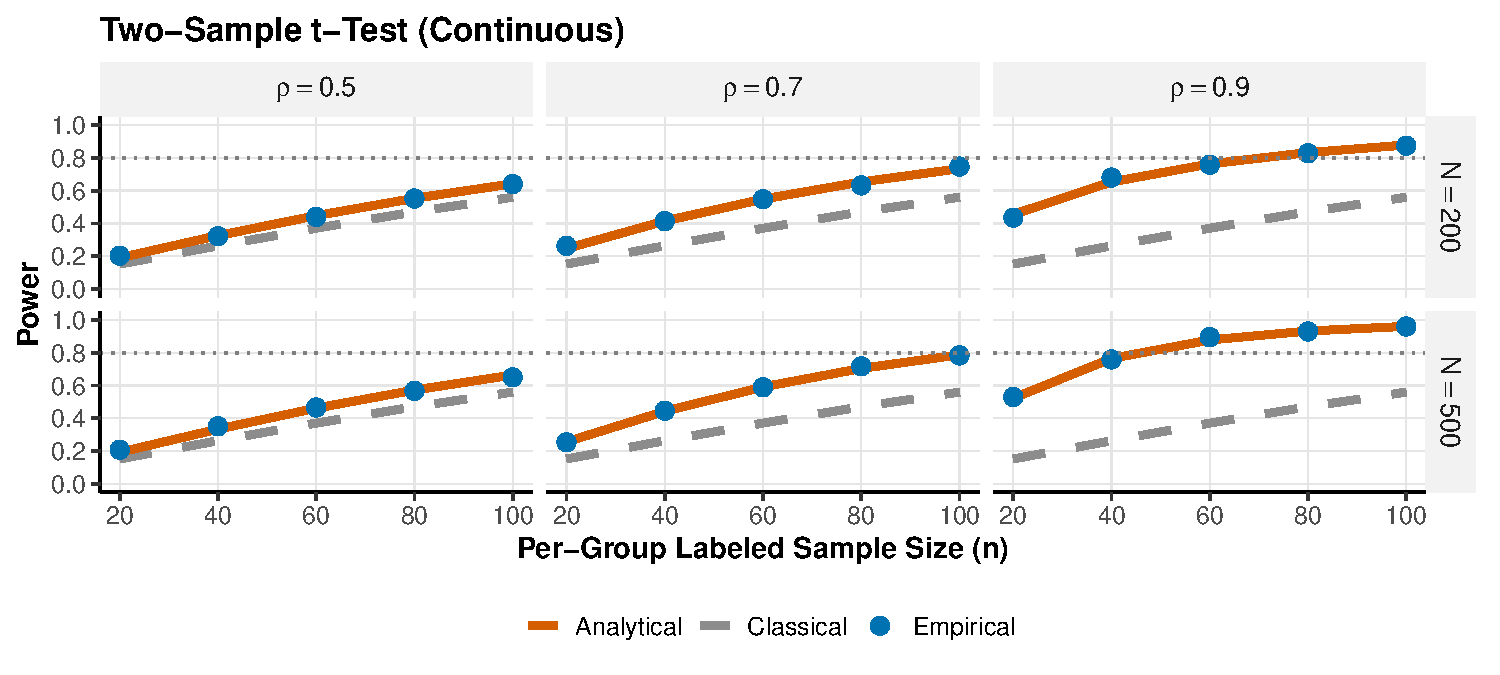
\includegraphics[width=0.95\linewidth]{figures/fig_validation_C_ttest_continuous.pdf}
\caption{Two-sample $t$-test with continuous Gaussian
  outcomes.  Analytical (lines) versus empirical (points) power.}
\label{fig:setting-C}
\end{figure}

\begin{figure}[!ht]
\centering
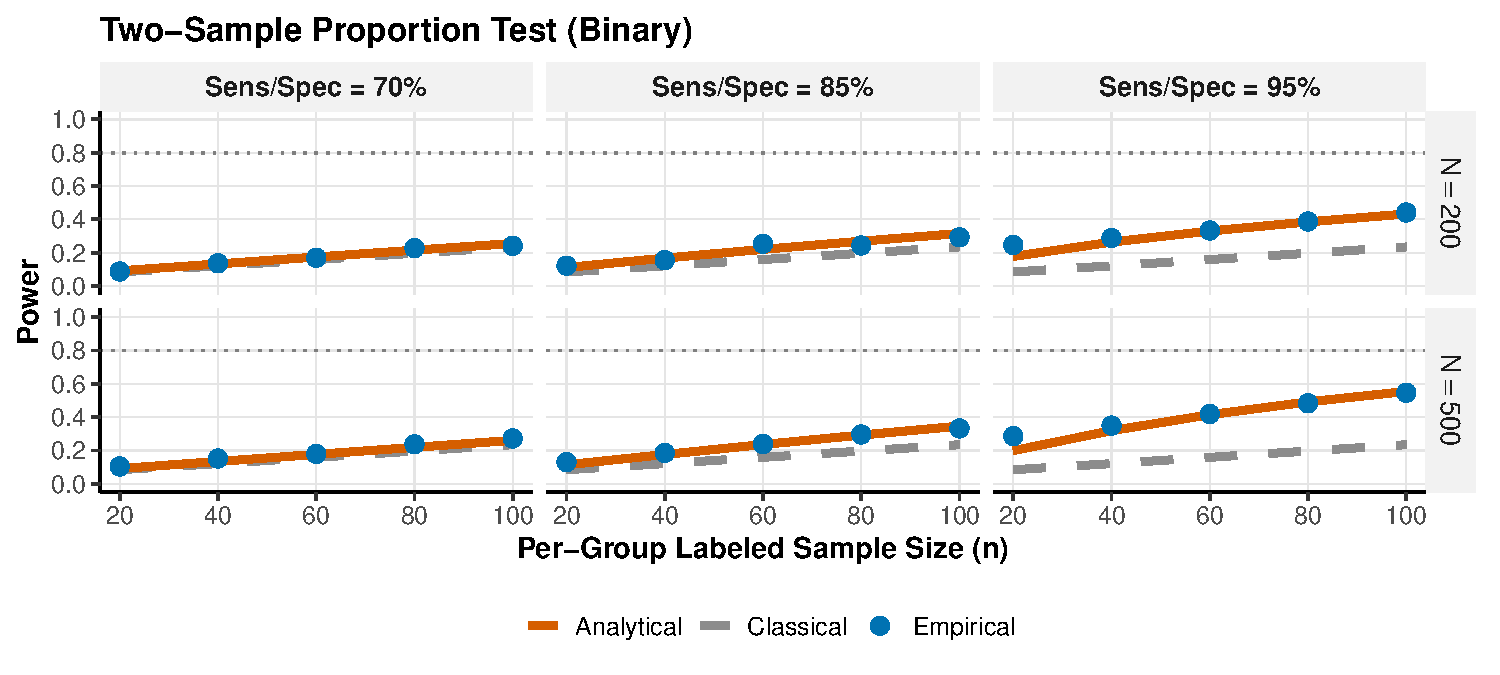
\includegraphics[width=0.95\linewidth]{figures/fig_validation_D_ttest_binary.pdf}
\caption{Two-sample proportion test with binary outcomes.
  Analytical (lines) versus empirical (points) power.}
\label{fig:setting-D}
\end{figure}

\begin{figure}[!ht]
\centering
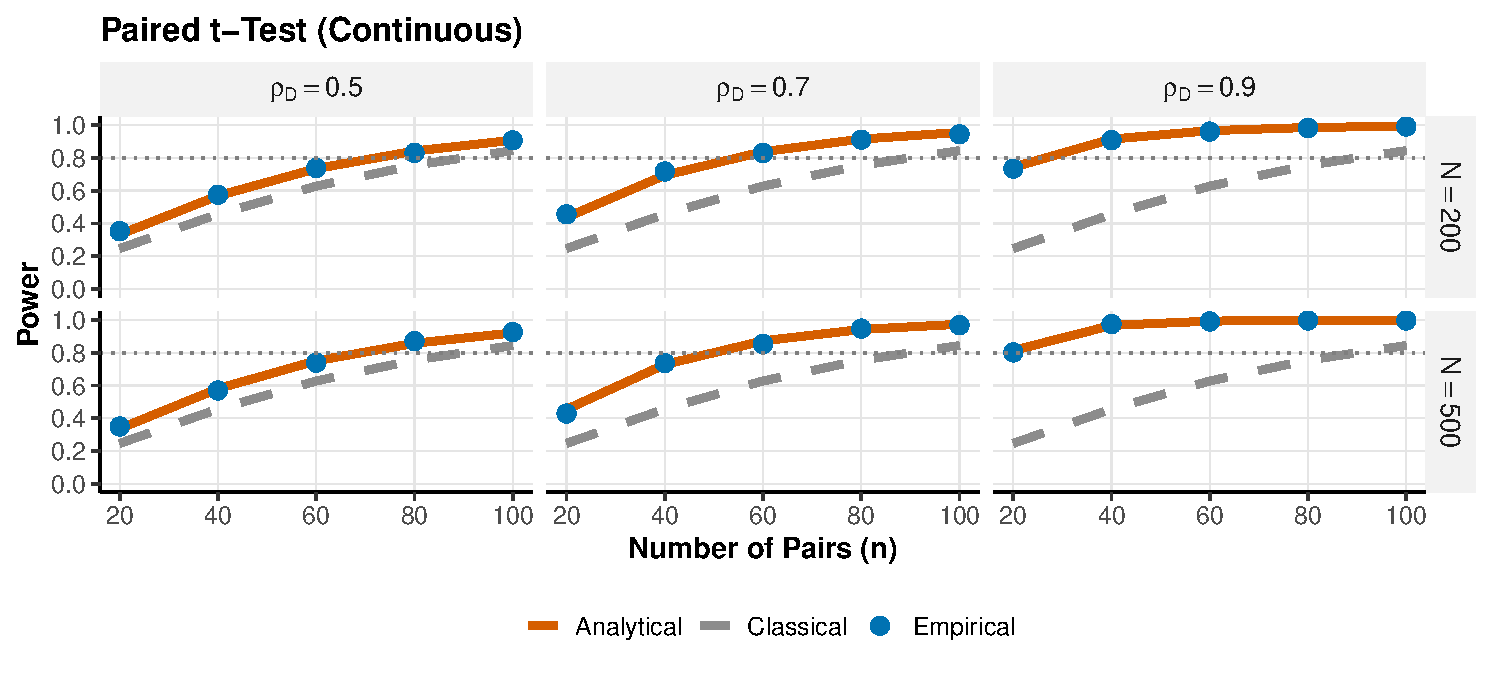
\includegraphics[width=0.95\linewidth]{figures/fig_validation_E_paired_continuous.pdf}
\caption{Paired $t$-test with continuous differences.
  Analytical (lines) versus empirical (points) power.}
\label{fig:setting-E}
\end{figure}

\begin{figure}[!ht]
\centering
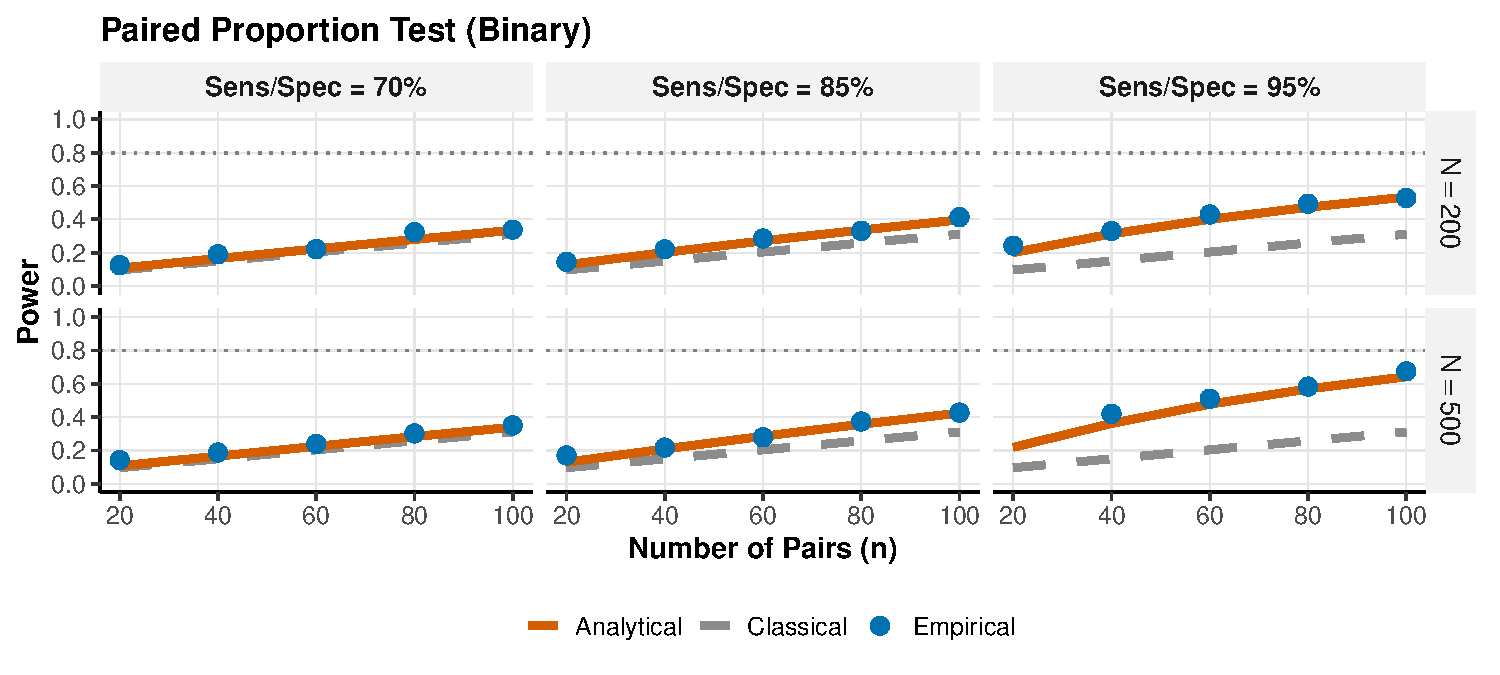
\includegraphics[width=0.95\linewidth]{figures/fig_validation_F_paired_binary.pdf}
\caption{Paired proportion test with binary differences.
  Analytical (lines) versus empirical (points) power.}
\label{fig:setting-F}
\end{figure}

\paragraph{Auxiliary planning checks.}

\paragraph{Sample-size inversion.}
For continuous one-sample means, binary one-sample means, continuous
two-sample means, and paired continuous designs, we fix target powers
in $\{0.60, 0.70, 0.80, 0.90\}$ and verify that the computed
$n^\star$ achieves power close to the target.  Figure~\ref{fig:setting-J}
plots achieved power minus target power, so exact inversion
corresponds to zero.  Each point is one design configuration within a
test family, such as a particular $\rho$ or binary-surrogate
accuracy, evaluated at the integer $n^\star$ returned by the
planning formula.  The analytical points recompute the asymptotic
power at that integer $n^\star$, while the empirical points are Monte
Carlo rejection rates at the same $n^\star$, so neither series is
forced to equal the target exactly.  Analytical deviations are
uniformly small, while empirical deviations are somewhat larger in the
smallest-$n$ configurations.  Some high-power binary targets at
$N = 500$ required $n^\star > N$ under the fixed-pool convention used
in the planning code and therefore do not appear.

\begin{figure}[!ht]
\centering
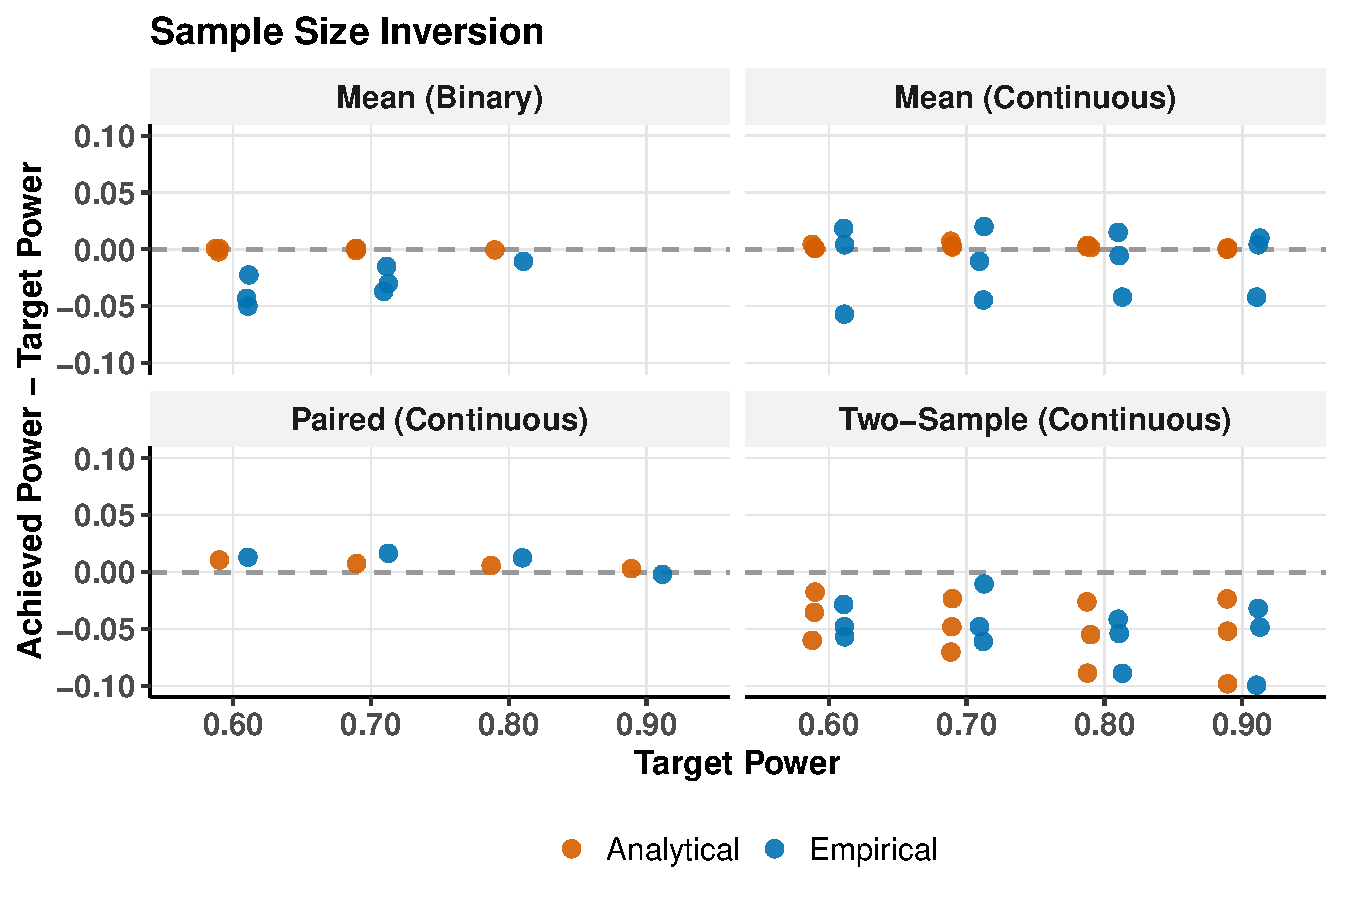
\includegraphics[width=0.95\linewidth]{figures/fig_validation_J_n_inversion.pdf}
\caption{Sample-size inversion check across one-sample, two-sample,
  and paired designs.  Points show achieved power minus target power
  at the planned integer $n^\star$; exact inversion would lie on the
  horizontal zero line.}
\label{fig:setting-J}
\end{figure}

\paragraph{Rule-of-thumb validation.}
We sweep $\rho \in [0.1, 0.99]$ and
$N \in \{200, 500, 1{,}000, 5{,}000\}$.  Rather than plotting the raw
ratio $n_{\mathrm{PPI}}/n_{\mathrm{cl}}$, Figure~\ref{fig:setting-K}
shows its deviation from the rule-of-thumb approximation
$1 - \rho^2$.  The error shrinks toward zero as $N$ grows, confirming
Corollary~\ref{cor:rule-of-thumb}.

\begin{figure}[!ht]
\centering
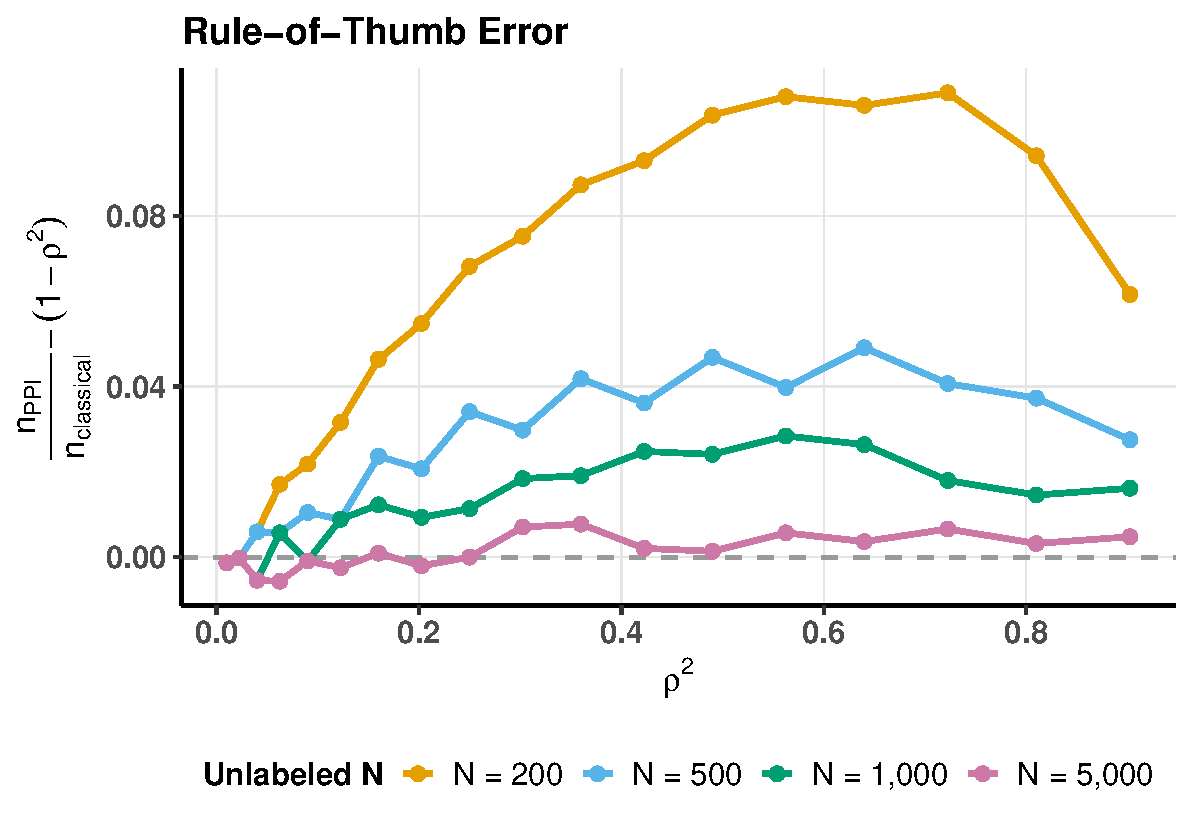
\includegraphics[width=0.95\linewidth]{figures/fig_validation_K_rule_of_thumb.pdf}
\caption{Rule-of-thumb error for the labeled-sample reduction ratio.
  Curves plot $n_{\mathrm{PPI}}/n_{\mathrm{cl}} - (1 - \rho^2)$
  against $\rho^2$ for several unlabeled-sample sizes $N$.}
\label{fig:setting-K}
\end{figure}

\paragraph{Type~I error calibration.}
We repeat the core one-sample, two-sample, paired, and
distributional-robustness experiments under the null ($\Delta = 0$) with
$R = 2{,}000$ replicates.  Observed \texttt{PPI++} rejection rates are
close to the nominal level: continuous settings range from 0.044 to
0.061, and binary settings from 0.044 to 0.060.  Figure~\ref{fig:setting-L}
shows the continuous null settings; the binary calibration results are
summarized here by their observed range.

\begin{figure}[!ht]
\centering
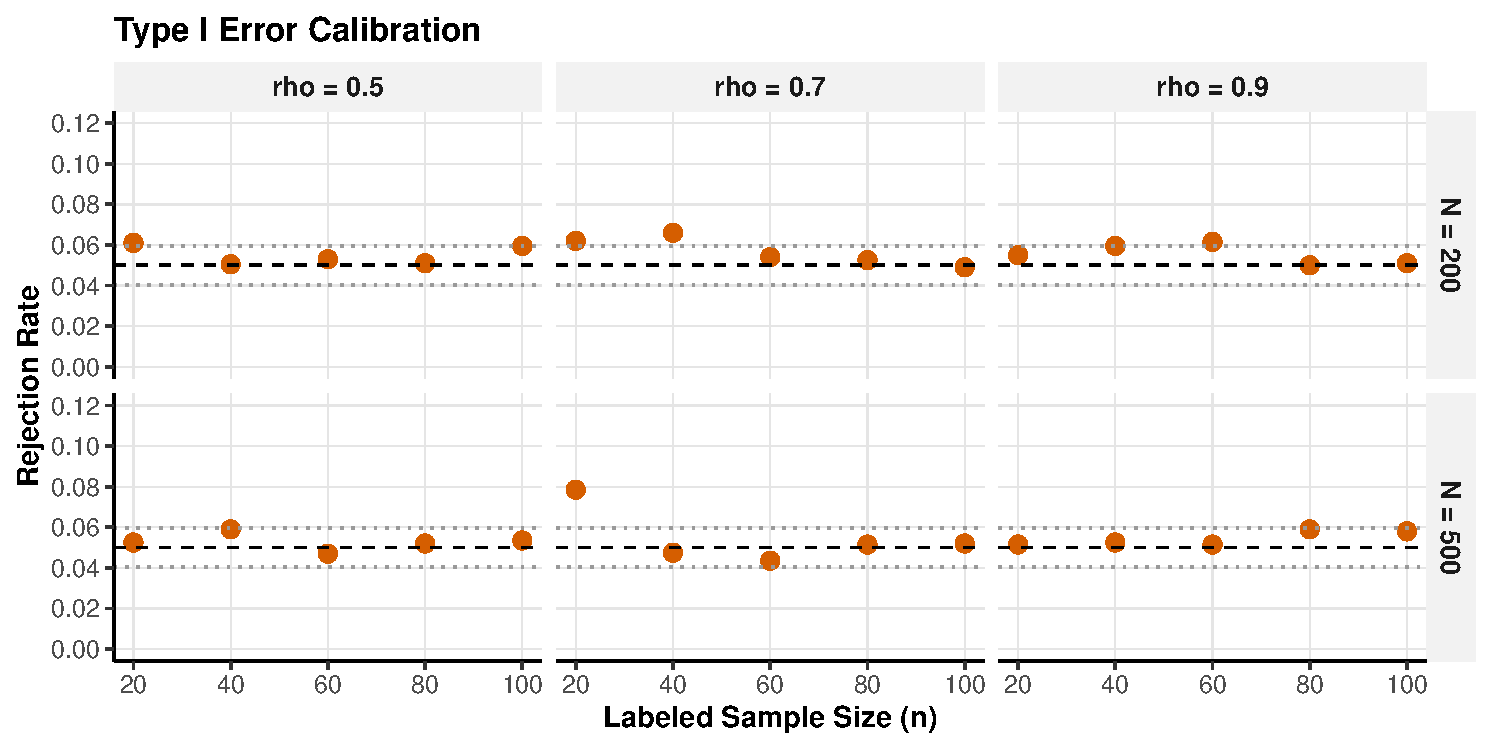
\includegraphics[width=0.95\linewidth]{figures/fig_validation_L_type1_continuous.pdf}
\caption{Type~I error calibration for the continuous null settings.
  Rejection rates remain close to the nominal level 0.05, with dotted
  lines showing the corresponding Monte Carlo fluctuation band for
  $R = 2{,}000$ replicates.}
\label{fig:setting-L}
\end{figure}

\paragraph{Plugin $\lambda$ convergence.}
We verify that the plugin estimate $\hat\lambda$ (computed from
labeled-data sample moments) converges to the oracle $\lambda^\star$
as $n$ increases, with $N = 1{,}000$ fixed.  Figure~\ref{fig:setting-M}
reports the root-mean-squared error of $\hat\lambda$ relative to
$\lambda^\star$, which shrinks toward zero as $n$ grows.

\begin{figure}[!ht]
\centering
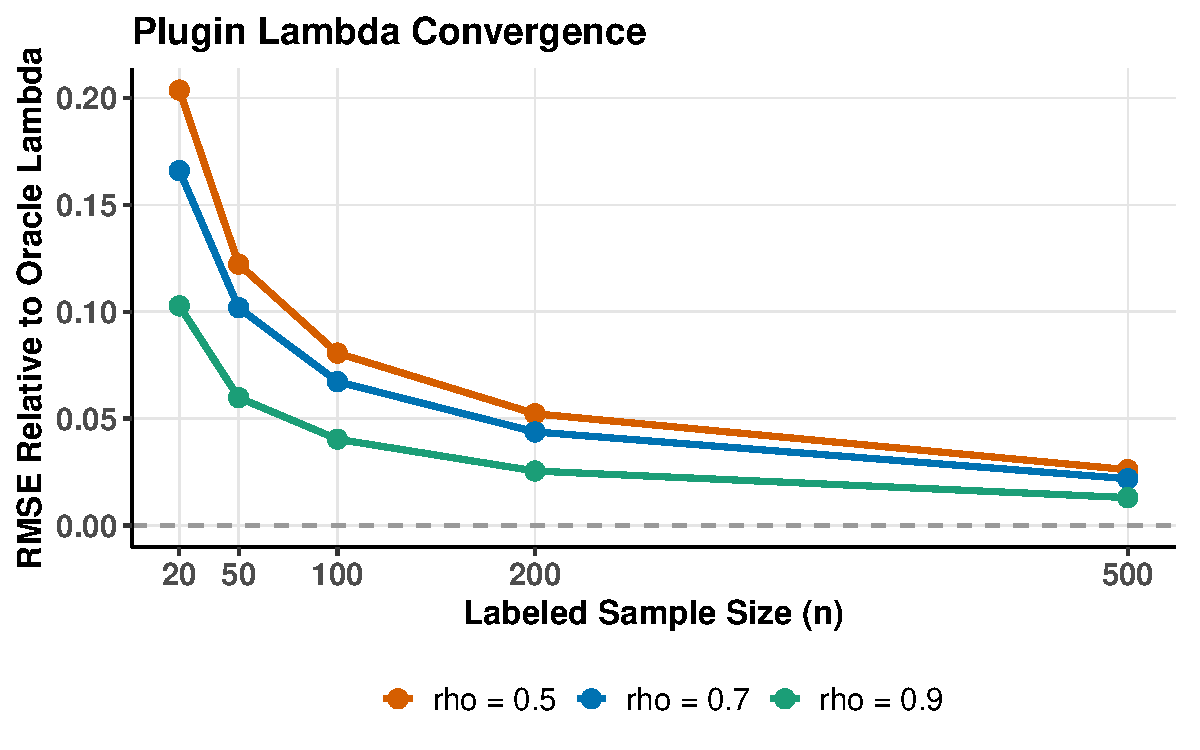
\includegraphics[width=0.95\linewidth]{figures/fig_validation_M_lambda_convergence.pdf}
\caption{Convergence of the plugin $\hat{\lambda}$ toward the oracle
  $\lambda^\star$ as the labeled sample size grows.  The plotted
  quantity is the root-mean-squared error relative to the oracle
  tuning value.}
\label{fig:setting-M}
\end{figure}

\paragraph{Robustness analyses.}

\paragraph{Plugin versus oracle $\lambda$.}
All previous robustness plots use the oracle $\lambda^\star$ computed
from the true population moments.  In practice, $\lambda$ must be
estimated from data.  This experiment reruns the Gaussian one-sample
DGP from the main validation grid on the same
$n \in \{20, 40, 60, 80, 100\}$ and $N \in \{200, 500\}$ grid, with
both the oracle and a plugin $\hat\lambda$ estimated from labeled-data
covariance.  Figure~\ref{fig:setting-N} shows that empirical power
under the plugin $\hat\lambda$ closely tracks the oracle empirical
curve; the analytical curve (based on the oracle variance) remains a
close approximation even at the smallest design point $n = 20$.
Quantitatively, the maximum discrepancy is 0.023 for oracle
$\lambda^\star$ and 0.037 for plugin $\hat\lambda$, while the
maximum oracle--plugin empirical difference is 0.031.

\begin{figure}[!ht]
\centering
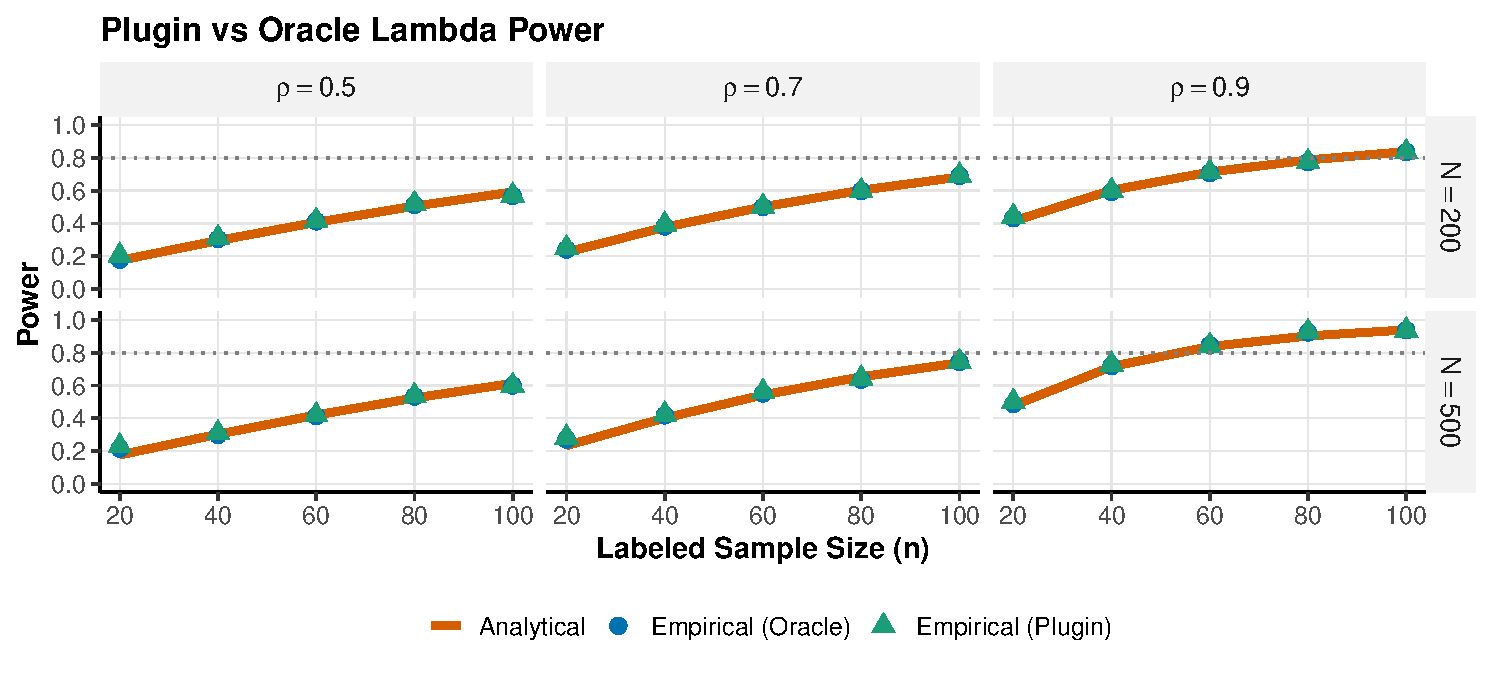
\includegraphics[width=0.95\linewidth]{figures/fig_validation_N_plugin_lambda.pdf}
\caption{Power with plugin versus oracle tuning.  The analytical curve
  uses the oracle variance formula, while the empirical points compare
  oracle and plugin versions of the \texttt{PPI++} test.}
\label{fig:setting-N}
\end{figure}

\paragraph{Power as a function of effect size.}
While the main validation figures fix $\Delta$ and vary $n$, it is also
standard to examine power as a function of effect size at fixed sample
sizes.  Here we sweep $\Delta \in [0, 0.5]$ for
$n \in \{20, 40, 60, 80, 100\}$ with $N = 500$.
Figure~\ref{fig:setting-O} displays the characteristic S-shaped
power curves; higher $\rho$ shifts the curve to the left, requiring
smaller $\Delta$ to achieve any given power level.  The maximum
discrepancy is 0.050.  This setting does not introduce a new variance
formula; it simply visualizes the same one-sample planning problem as
the main one-sample validation figures, but on an effect-size axis
rather than a sample-size axis.

\begin{figure}[!ht]
\centering
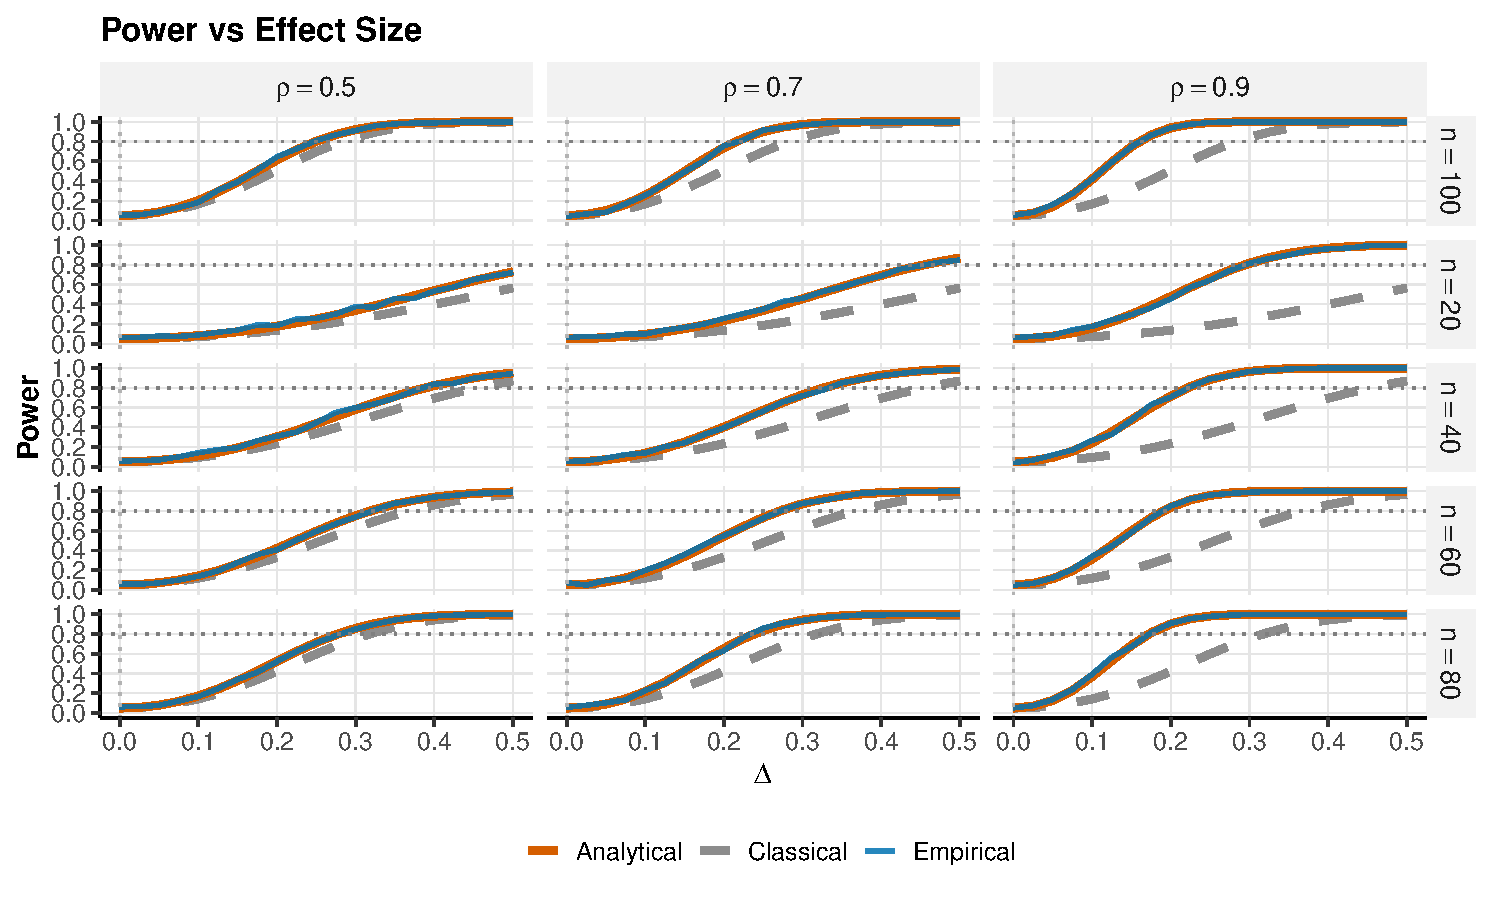
\includegraphics[width=0.95\linewidth]{figures/fig_validation_O_power_vs_delta.pdf}
\caption{Power as a function of effect size for the Gaussian
  one-sample mean problem.  Higher prediction quality shifts the
  \texttt{PPI++} curve leftward relative to the classical design.}
\label{fig:setting-O}
\end{figure}

\paragraph{Small labeled samples.}
The power formula relies on the normal approximation, which may be
inaccurate when $n$ is very small.  Here we push to
$n \in \{15, 20, 25, 30, 50, 100\}$ with $R = 2{,}000$ replicates
for tighter Monte Carlo estimates.  Figure~\ref{fig:setting-P}
shows that the analytical formula remains usable for Gaussian
outcomes even at small~$n$.  The maximum discrepancy is 0.036 for
$n \le 25$ and much smaller (0.009) for $n \ge 50$, suggesting that
the normal approximation is most reliable once $n$ is at least
moderate.

\begin{figure}[!ht]
\centering
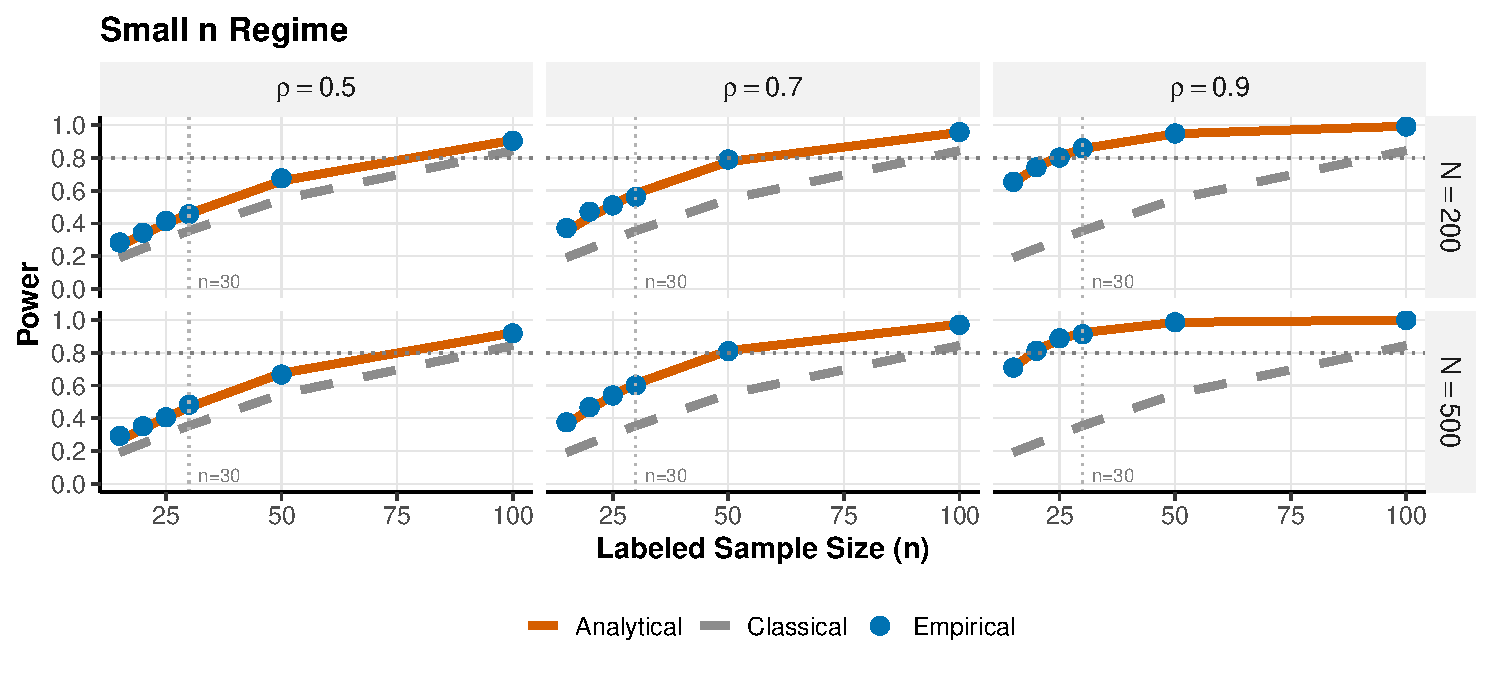
\includegraphics[width=0.95\linewidth]{figures/fig_validation_P_small_n.pdf}
\caption{Small-$n$ regime for the Gaussian one-sample mean problem.
  Agreement remains usable down to $n = 15$, with the largest
  discrepancies concentrated in the smallest labeled samples.}
\label{fig:setting-P}
\end{figure}

\paragraph{$N/n$ ratio sensitivity.}
Current PPI practice typically assumes $N \gg n$. Here we fix
$n = 50$ and vary $N/n$ from $1$ to $100$.
Figure~\ref{fig:setting-Q} reveals three findings.  First, at
$N/n = 1$, the \texttt{PPI++} power gain is smaller than in high-ratio
regimes but can still be material when $\rho$ is high.  Second, the
gain saturates: most of the benefit accrues by
$N/n \approx 10$--$20$.  Third, the gain is modulated by $\rho$:
at $\rho = 0.5$, even $N/n = 100$ provides only a modest
improvement, while at $\rho = 0.9$, the improvement is substantial.

\begin{figure}[!ht]
\centering
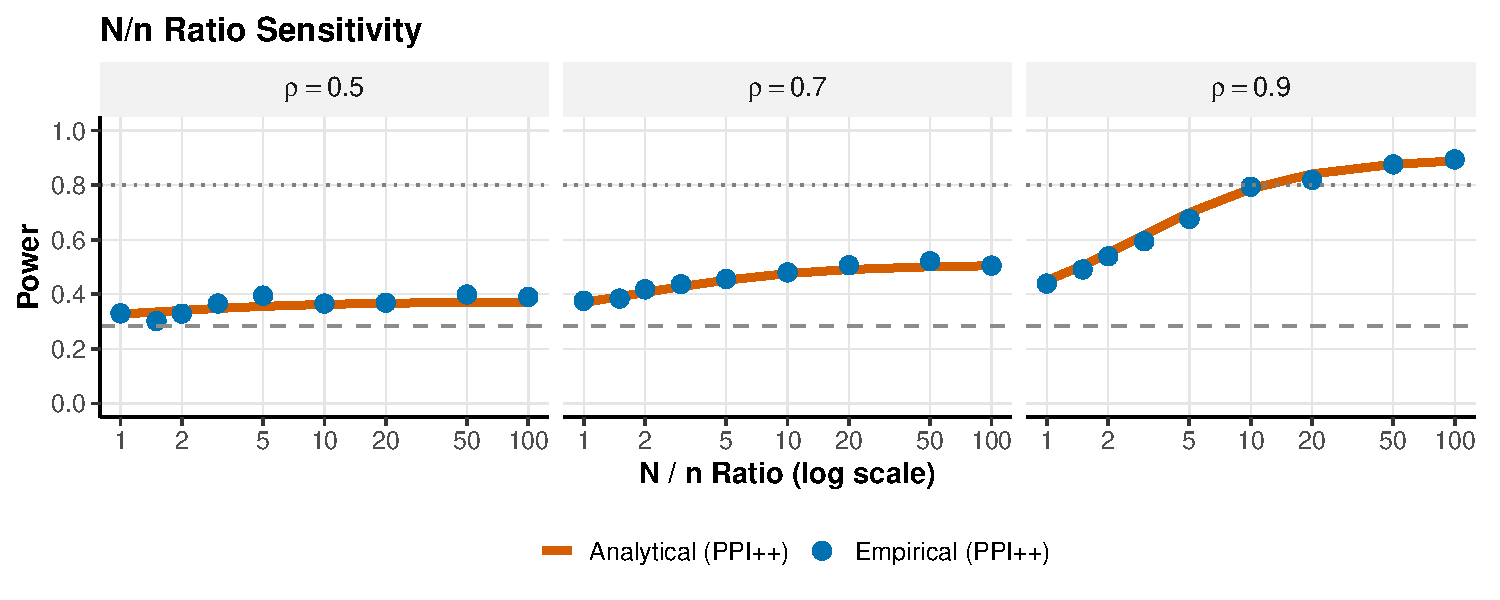
\includegraphics[width=0.95\linewidth]{figures/fig_validation_Q_Nn_ratio.pdf}
\caption{Sensitivity to the unlabeled-to-labeled ratio $N/n$.  Power
  gains increase quickly at first and then saturate once the
  unlabeled pool is moderately large.}
\label{fig:setting-Q}
\end{figure}

\paragraph{Unequal group sizes.}
Two-sample tests in practice often have unbalanced designs.
Here we fix the total labeled budget
($n_A + n_B = 100$, $N_A + N_B = 600$) and vary the allocation
ratio $n_A : n_B \in \{1{:}1, 1.5{:}1, 2{:}1, 3{:}1, 4{:}1\}$,
allocating the unlabeled totals in the same ratio so that
$N_A : N_B = n_A : n_B$.
Figure~\ref{fig:setting-R} shows that the analytical formula
accurately tracks empirical power across all ratios.  Power
decreases with increasing imbalance, consistent with the classical
result that balanced allocation maximizes power for a fixed total
budget.  The maximum discrepancy is 0.030.

\begin{figure}[!ht]
\centering
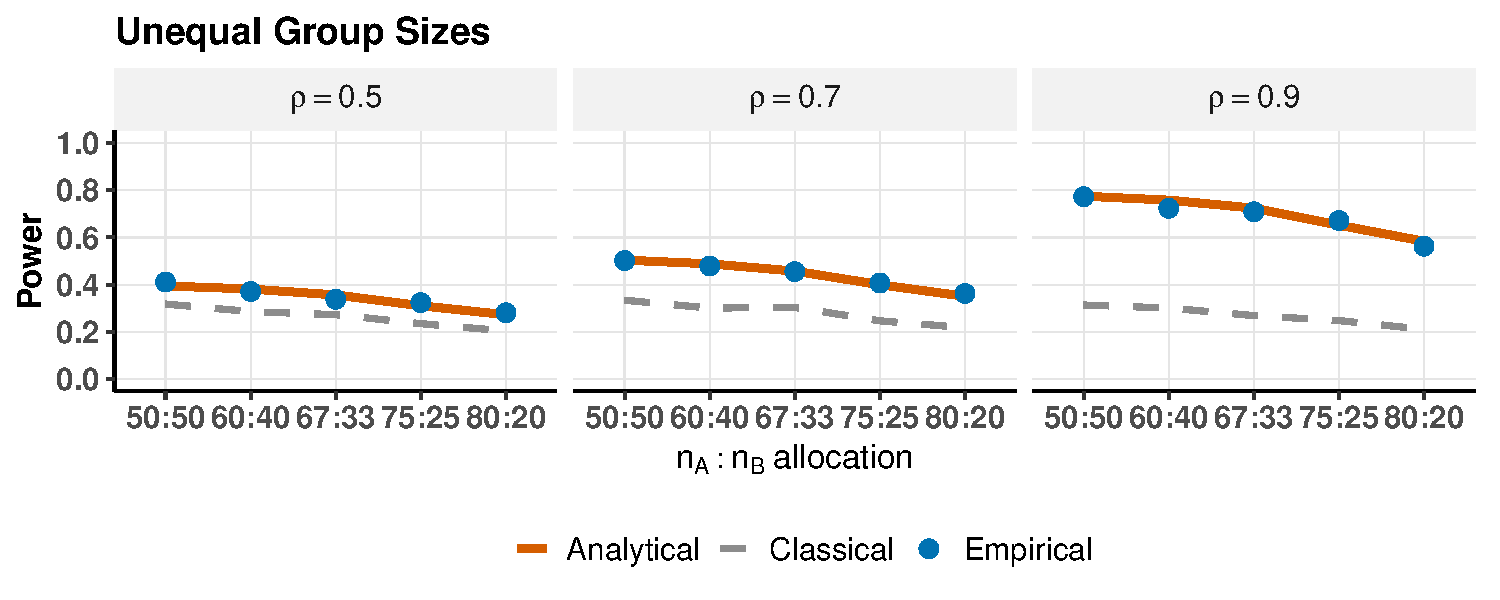
\includegraphics[width=0.95\linewidth]{figures/fig_validation_R_unequal_groups.pdf}
\caption{Unequal-group two-sample designs.  Power decreases with
  stronger allocation imbalance, while the analytical formula
  continues to track the empirical results closely.}
\label{fig:setting-R}
\end{figure}

\paragraph{Misspecified prediction quality.}
In practice, the user must specify $\rho_{Yf}$ at the planning stage
based on pilot data or published benchmarks, but the true correlation
may differ.  This experiment quantifies this sensitivity: for each
$\rho_{\mathrm{plan}} \in \{0.5, 0.7, 0.9\}$, we compute the
required $n^\star$ assuming $\rho_{\mathrm{plan}}$, then evaluate
the actual power at $n^\star$ under the true
$\rho_{\mathrm{true}} = \rho_{\mathrm{plan}} + \delta_\rho$ with
$\delta_\rho \in \{-0.20, -0.15, \ldots, 0.20\}$, retaining only
feasible values with $\rho_{\mathrm{true}} \in (0.01, 0.99)$, and
$R = 2{,}000$ replicates.  When
$\rho_{\mathrm{true}} < \rho_{\mathrm{plan}}$ (the predictor is
worse than expected), the study is underpowered.  Conversely, when
$\rho_{\mathrm{true}} > \rho_{\mathrm{plan}}$, the study is
conservatively overpowered.  This asymmetry suggests that
practitioners should use conservative (lower-bound) estimates of
prediction quality when planning studies, analogous to the common
advice to use conservative effect-size estimates in classical power
analysis.

\begin{figure}[!ht]
\centering
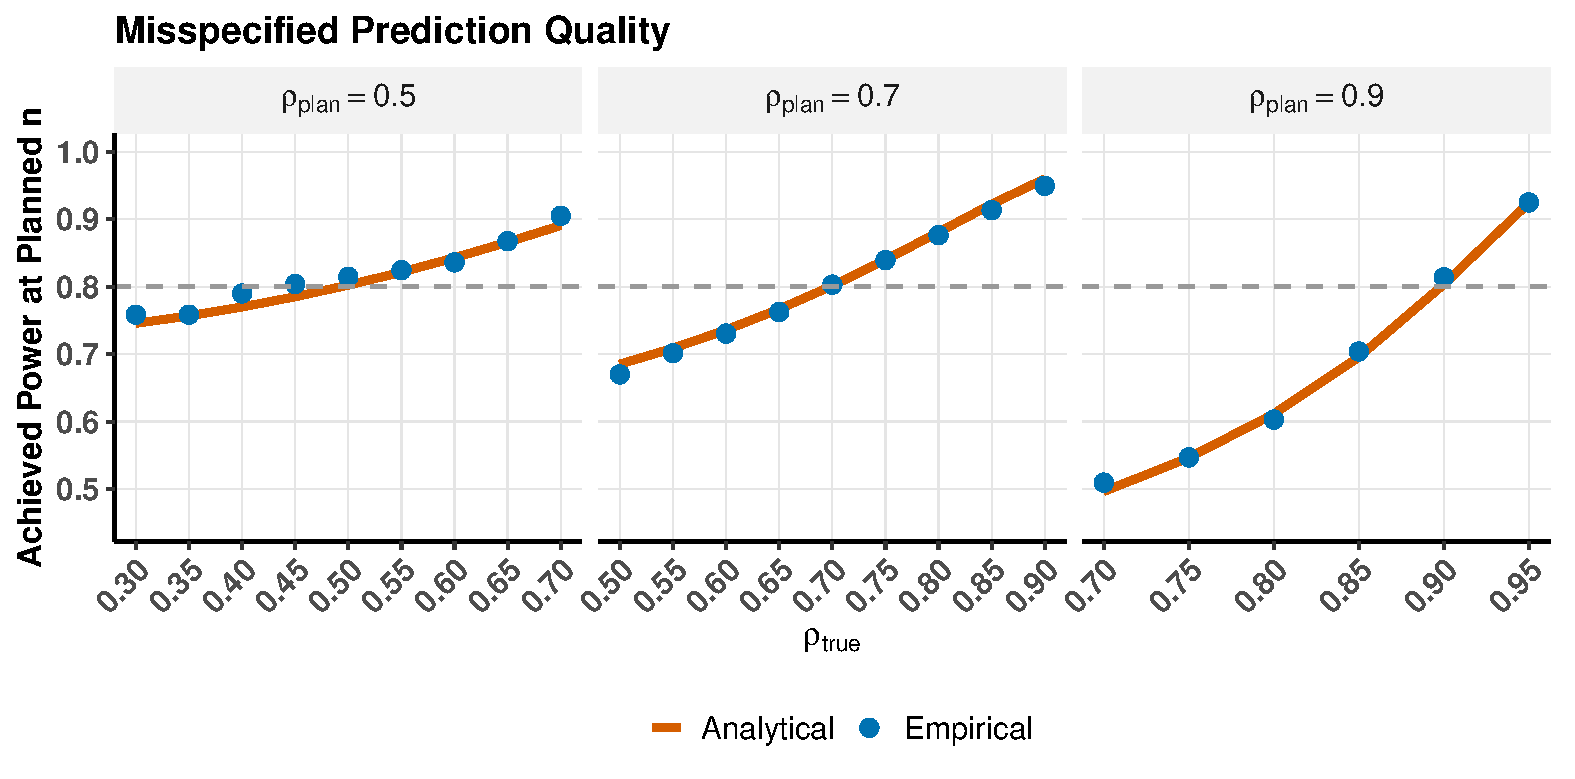
\includegraphics[width=0.95\linewidth]{figures/fig_validation_setting19_misspecified_rho.pdf}
\caption{Sensitivity to misspecified prediction quality.  The dashed
  line marks the target power, while each panel varies the true
  prediction quality around the value used at the planning stage.}
\label{fig:setting-19}
\end{figure}

\paragraph{Distributional robustness.}

Log-normal (right-skewed) and $t_5$ (heavy-tailed) outcomes probe how
far the Gaussian approximation can
be pushed.  For $t_5$ outcomes, agreement remains tight, whereas the
log-normal setting shows larger discrepancies in the most skewed,
small-$n$ regime; see Figure~\ref{fig:setting-GH}.

\begin{figure}[!ht]
\centering
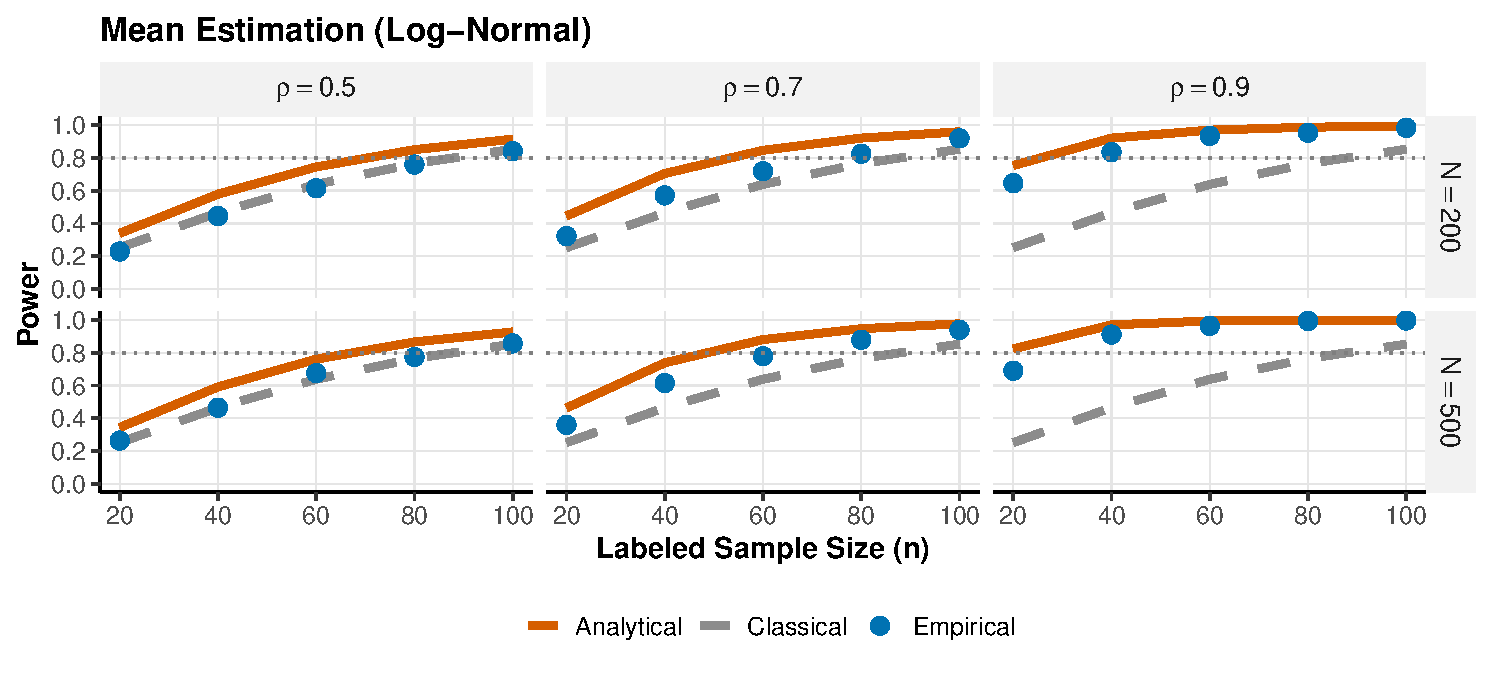
\includegraphics[width=0.95\linewidth]{figures/fig_validation_G_lognormal.pdf}
\vspace{0.4em}
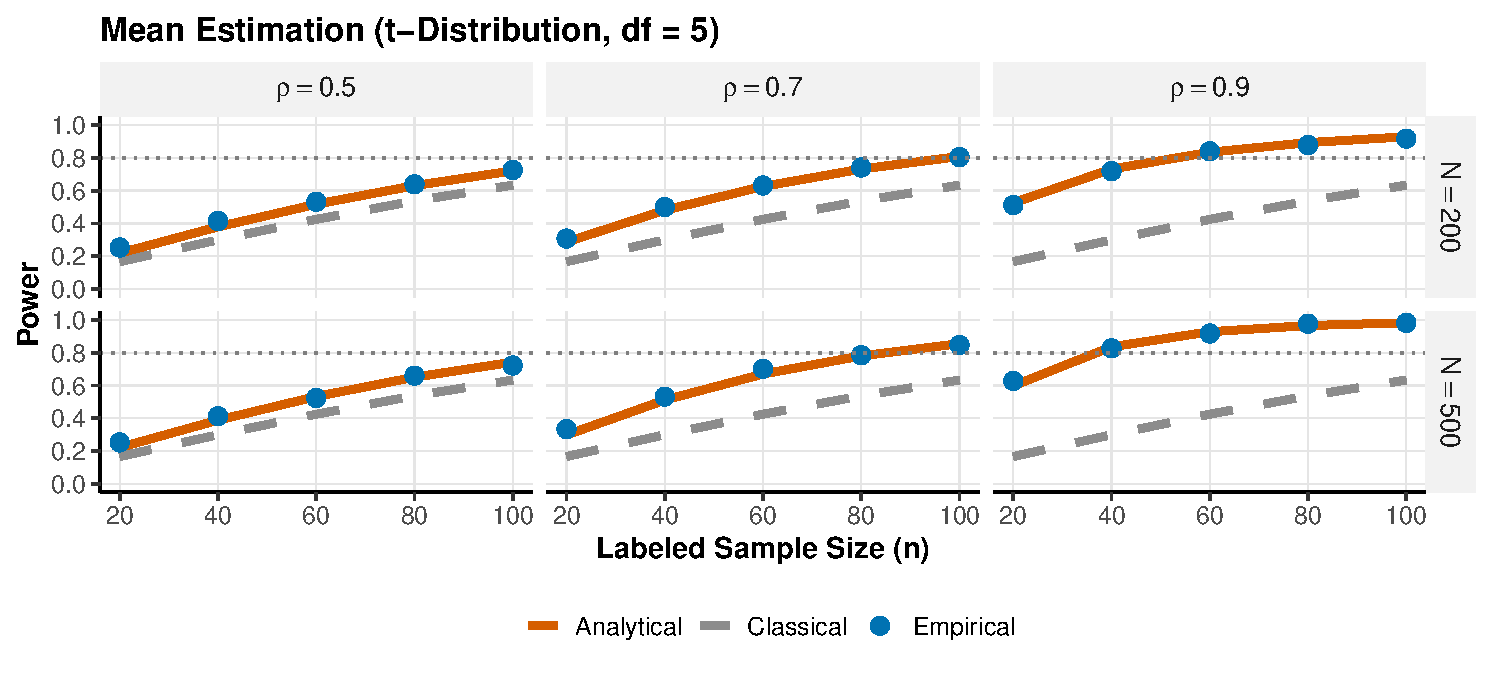
\includegraphics[width=0.95\linewidth]{figures/fig_validation_H_tdist.pdf}
\caption{Distributional robustness for the one-sample mean problem.
  Top: log-normal outcomes, where the CLT-based formula overshoots at
  small~$n$ under severe skew (max discrepancy 0.144 at $n = 50$,
  $\rho = 0.5$). Bottom: $t_5$ outcomes, where agreement remains tight
  despite heavy tails (max discrepancy 0.018).}
\label{fig:setting-GH}
\end{figure}
